\subsection{Amplificatore invertente}
Schema amplificatore invertente:
%inserire circuito
Le resistenze sono state scelte in modo da avere guadagno $A=-10 \frac{V}{V}$
$R_1=9.85 \pm 0.05\,k\Omega $%mettere errore
$R_2=101.3 \pm 0.6\,k\Omega$ %mettere errore
$R_3=56.0 \pm 0.3\,\Omega$ %mettere errore

\subsubsection{Calcolo amplificazione}
Dimostrazione che amplificazione in configurazione invertente è data da %inserire dimostrazione

\subsubsection{Analisi}
La stima di A teorica, a partire dalle resistenze misurate è:
$A_{teorica}=$ %inserire valore teorico

Le misure sono state fatte applicando una tensione sinusoidale di frequenza $ f=1 \,kHz$, variando l'ampiezza tra 
$0.2 V_{pp}$ e $4 V_{pp}$.

\begin{grafico} 
 \centering 
 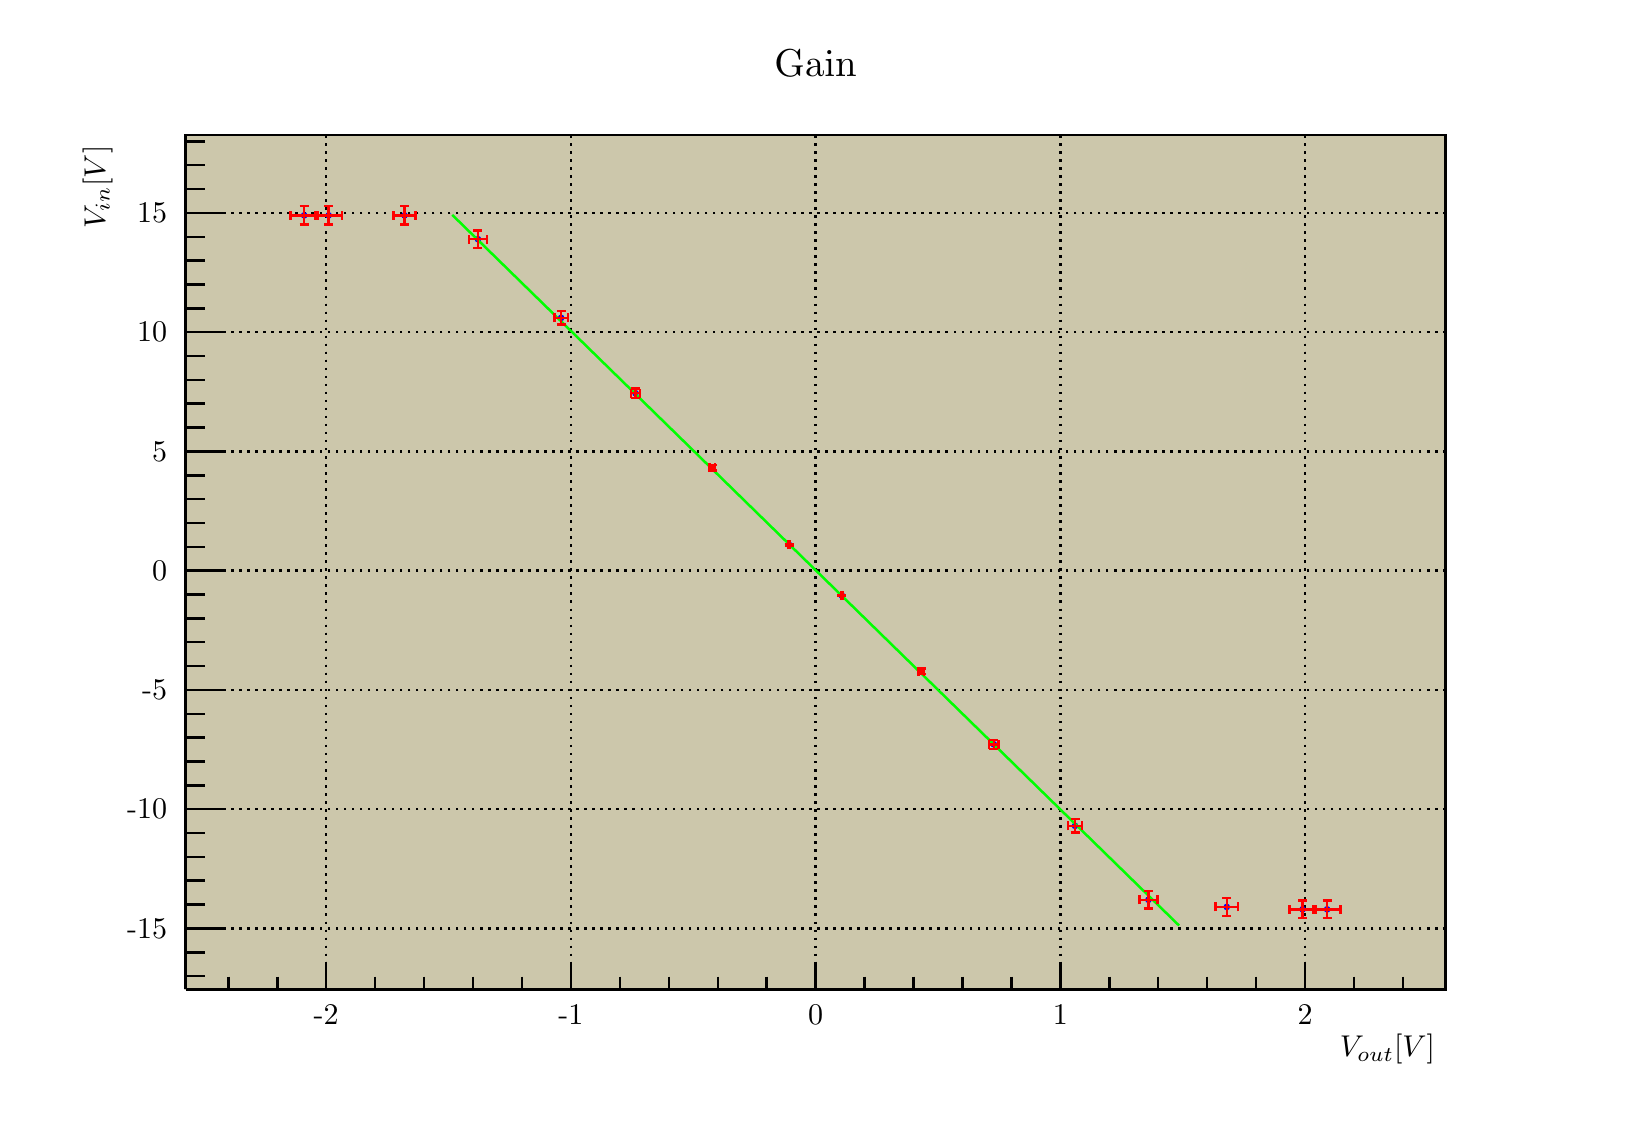
\begin{tikzpicture}
\pgfdeclareplotmark{cross} {
\pgfpathmoveto{\pgfpoint{-0.3\pgfplotmarksize}{\pgfplotmarksize}}
\pgfpathlineto{\pgfpoint{+0.3\pgfplotmarksize}{\pgfplotmarksize}}
\pgfpathlineto{\pgfpoint{+0.3\pgfplotmarksize}{0.3\pgfplotmarksize}}
\pgfpathlineto{\pgfpoint{+1\pgfplotmarksize}{0.3\pgfplotmarksize}}
\pgfpathlineto{\pgfpoint{+1\pgfplotmarksize}{-0.3\pgfplotmarksize}}
\pgfpathlineto{\pgfpoint{+0.3\pgfplotmarksize}{-0.3\pgfplotmarksize}}
\pgfpathlineto{\pgfpoint{+0.3\pgfplotmarksize}{-1.\pgfplotmarksize}}
\pgfpathlineto{\pgfpoint{-0.3\pgfplotmarksize}{-1.\pgfplotmarksize}}
\pgfpathlineto{\pgfpoint{-0.3\pgfplotmarksize}{-0.3\pgfplotmarksize}}
\pgfpathlineto{\pgfpoint{-1.\pgfplotmarksize}{-0.3\pgfplotmarksize}}
\pgfpathlineto{\pgfpoint{-1.\pgfplotmarksize}{0.3\pgfplotmarksize}}
\pgfpathlineto{\pgfpoint{-0.3\pgfplotmarksize}{0.3\pgfplotmarksize}}
\pgfpathclose
\pgfusepathqstroke
}
\pgfdeclareplotmark{cross*} {
\pgfpathmoveto{\pgfpoint{-0.3\pgfplotmarksize}{\pgfplotmarksize}}
\pgfpathlineto{\pgfpoint{+0.3\pgfplotmarksize}{\pgfplotmarksize}}
\pgfpathlineto{\pgfpoint{+0.3\pgfplotmarksize}{0.3\pgfplotmarksize}}
\pgfpathlineto{\pgfpoint{+1\pgfplotmarksize}{0.3\pgfplotmarksize}}
\pgfpathlineto{\pgfpoint{+1\pgfplotmarksize}{-0.3\pgfplotmarksize}}
\pgfpathlineto{\pgfpoint{+0.3\pgfplotmarksize}{-0.3\pgfplotmarksize}}
\pgfpathlineto{\pgfpoint{+0.3\pgfplotmarksize}{-1.\pgfplotmarksize}}
\pgfpathlineto{\pgfpoint{-0.3\pgfplotmarksize}{-1.\pgfplotmarksize}}
\pgfpathlineto{\pgfpoint{-0.3\pgfplotmarksize}{-0.3\pgfplotmarksize}}
\pgfpathlineto{\pgfpoint{-1.\pgfplotmarksize}{-0.3\pgfplotmarksize}}
\pgfpathlineto{\pgfpoint{-1.\pgfplotmarksize}{0.3\pgfplotmarksize}}
\pgfpathlineto{\pgfpoint{-0.3\pgfplotmarksize}{0.3\pgfplotmarksize}}
\pgfpathclose
\pgfusepathqfillstroke
}
\pgfdeclareplotmark{newstar} {
\pgfpathmoveto{\pgfqpoint{0pt}{\pgfplotmarksize}}
\pgfpathlineto{\pgfqpointpolar{44}{0.5\pgfplotmarksize}}
\pgfpathlineto{\pgfqpointpolar{18}{\pgfplotmarksize}}
\pgfpathlineto{\pgfqpointpolar{-20}{0.5\pgfplotmarksize}}
\pgfpathlineto{\pgfqpointpolar{-54}{\pgfplotmarksize}}
\pgfpathlineto{\pgfqpointpolar{-90}{0.5\pgfplotmarksize}}
\pgfpathlineto{\pgfqpointpolar{234}{\pgfplotmarksize}}
\pgfpathlineto{\pgfqpointpolar{198}{0.5\pgfplotmarksize}}
\pgfpathlineto{\pgfqpointpolar{162}{\pgfplotmarksize}}
\pgfpathlineto{\pgfqpointpolar{134}{0.5\pgfplotmarksize}}
\pgfpathclose
\pgfusepathqstroke
}
\pgfdeclareplotmark{newstar*} {
\pgfpathmoveto{\pgfqpoint{0pt}{\pgfplotmarksize}}
\pgfpathlineto{\pgfqpointpolar{44}{0.5\pgfplotmarksize}}
\pgfpathlineto{\pgfqpointpolar{18}{\pgfplotmarksize}}
\pgfpathlineto{\pgfqpointpolar{-20}{0.5\pgfplotmarksize}}
\pgfpathlineto{\pgfqpointpolar{-54}{\pgfplotmarksize}}
\pgfpathlineto{\pgfqpointpolar{-90}{0.5\pgfplotmarksize}}
\pgfpathlineto{\pgfqpointpolar{234}{\pgfplotmarksize}}
\pgfpathlineto{\pgfqpointpolar{198}{0.5\pgfplotmarksize}}
\pgfpathlineto{\pgfqpointpolar{162}{\pgfplotmarksize}}
\pgfpathlineto{\pgfqpointpolar{134}{0.5\pgfplotmarksize}}
\pgfpathclose
\pgfusepathqfillstroke
}
\definecolor{c}{rgb}{1,1,1};
\draw [color=c, fill=c] (0,0) rectangle (20,13.5632);
\definecolor{c}{rgb}{0.8,0.78,0.67};
\draw [color=c, fill=c] (2,1.35632) rectangle (18,12.2069);
\definecolor{c}{rgb}{0,0,0};
\draw [c,line width=0.9] (2,1.35632) -- (2,12.2069) -- (18,12.2069) -- (18,1.35632) -- (2,1.35632);
\definecolor{c}{rgb}{0.8,0.78,0.67};
\draw [color=c, fill=c] (2,1.35632) rectangle (18,12.2069);
\definecolor{c}{rgb}{0,0,0};
\draw [c,line width=0.9] (2,1.35632) -- (2,12.2069) -- (18,12.2069) -- (18,1.35632) -- (2,1.35632);
\draw [c,line width=0.9] (2,1.35632) -- (18,1.35632);
\draw [c,dotted,line width=0.9] (3.78447,12.2069) -- (3.78447,1.35632);
\draw [c,dotted,line width=0.9] (6.89224,12.2069) -- (6.89224,1.35632);
\draw [c,dotted,line width=0.9] (10,12.2069) -- (10,1.35632);
\draw [c,dotted,line width=0.9] (13.1078,12.2069) -- (13.1078,1.35632);
\draw [c,dotted,line width=0.9] (16.2155,12.2069) -- (16.2155,1.35632);
\draw [c,dotted,line width=0.9] (3.78447,12.2069) -- (3.78447,1.35632);
\draw [c,dotted,line width=0.9] (16.2155,12.2069) -- (16.2155,1.35632);
\draw [c,line width=0.9] (2,1.35632) -- (2,12.2069);
\draw [c,dotted,line width=0.9] (18,2.13085) -- (2,2.13085);
\draw [c,dotted,line width=0.9] (18,3.64523) -- (2,3.64523);
\draw [c,dotted,line width=0.9] (18,5.1596) -- (2,5.1596);
\draw [c,dotted,line width=0.9] (18,6.67397) -- (2,6.67397);
\draw [c,dotted,line width=0.9] (18,8.18834) -- (2,8.18834);
\draw [c,dotted,line width=0.9] (18,9.70271) -- (2,9.70271);
\draw [c,dotted,line width=0.9] (18,11.2171) -- (2,11.2171);
\draw [c,dotted,line width=0.9] (18,2.13085) -- (2,2.13085);
\draw [c,dotted,line width=0.9] (18,11.2171) -- (2,11.2171);
\draw [c,line width=0.9] (2,1.35632) -- (18,1.35632);
\draw [anchor= east] (18,0.596782) node[scale=1.08496, color=c, rotate=0]{$V_{out} [V]$};
\draw [c,line width=0.9] (3.78447,1.68184) -- (3.78447,1.35632);
\draw [c,line width=0.9] (4.40603,1.51908) -- (4.40603,1.35632);
\draw [c,line width=0.9] (5.02758,1.51908) -- (5.02758,1.35632);
\draw [c,line width=0.9] (5.64913,1.51908) -- (5.64913,1.35632);
\draw [c,line width=0.9] (6.27068,1.51908) -- (6.27068,1.35632);
\draw [c,line width=0.9] (6.89224,1.68184) -- (6.89224,1.35632);
\draw [c,line width=0.9] (7.51379,1.51908) -- (7.51379,1.35632);
\draw [c,line width=0.9] (8.13534,1.51908) -- (8.13534,1.35632);
\draw [c,line width=0.9] (8.7569,1.51908) -- (8.7569,1.35632);
\draw [c,line width=0.9] (9.37845,1.51908) -- (9.37845,1.35632);
\draw [c,line width=0.9] (10,1.68184) -- (10,1.35632);
\draw [c,line width=0.9] (10.6216,1.51908) -- (10.6216,1.35632);
\draw [c,line width=0.9] (11.2431,1.51908) -- (11.2431,1.35632);
\draw [c,line width=0.9] (11.8647,1.51908) -- (11.8647,1.35632);
\draw [c,line width=0.9] (12.4862,1.51908) -- (12.4862,1.35632);
\draw [c,line width=0.9] (13.1078,1.68184) -- (13.1078,1.35632);
\draw [c,line width=0.9] (13.7293,1.51908) -- (13.7293,1.35632);
\draw [c,line width=0.9] (14.3509,1.51908) -- (14.3509,1.35632);
\draw [c,line width=0.9] (14.9724,1.51908) -- (14.9724,1.35632);
\draw [c,line width=0.9] (15.594,1.51908) -- (15.594,1.35632);
\draw [c,line width=0.9] (16.2155,1.68184) -- (16.2155,1.35632);
\draw [c,line width=0.9] (3.78447,1.68184) -- (3.78447,1.35632);
\draw [c,line width=0.9] (3.16292,1.51908) -- (3.16292,1.35632);
\draw [c,line width=0.9] (2.54137,1.51908) -- (2.54137,1.35632);
\draw [c,line width=0.9] (16.2155,1.68184) -- (16.2155,1.35632);
\draw [c,line width=0.9] (16.8371,1.51908) -- (16.8371,1.35632);
\draw [c,line width=0.9] (17.4586,1.51908) -- (17.4586,1.35632);
\draw [anchor=base] (3.78447,0.908736) node[scale=1.08496, color=c, rotate=0]{-2};
\draw [anchor=base] (6.89224,0.908736) node[scale=1.08496, color=c, rotate=0]{-1};
\draw [anchor=base] (10,0.908736) node[scale=1.08496, color=c, rotate=0]{0};
\draw [anchor=base] (13.1078,0.908736) node[scale=1.08496, color=c, rotate=0]{1};
\draw [anchor=base] (16.2155,0.908736) node[scale=1.08496, color=c, rotate=0]{2};
\draw [c,line width=0.9] (2,1.35632) -- (2,12.2069);
\draw [anchor= east] (0.88,12.2069) node[scale=1.08496, color=c, rotate=90]{$V_{in} [V]$};
\draw [c,line width=0.9] (2.48,2.13085) -- (2,2.13085);
\draw [c,line width=0.9] (2.24,2.43373) -- (2,2.43373);
\draw [c,line width=0.9] (2.24,2.7366) -- (2,2.7366);
\draw [c,line width=0.9] (2.24,3.03948) -- (2,3.03948);
\draw [c,line width=0.9] (2.24,3.34235) -- (2,3.34235);
\draw [c,line width=0.9] (2.48,3.64523) -- (2,3.64523);
\draw [c,line width=0.9] (2.24,3.9481) -- (2,3.9481);
\draw [c,line width=0.9] (2.24,4.25097) -- (2,4.25097);
\draw [c,line width=0.9] (2.24,4.55385) -- (2,4.55385);
\draw [c,line width=0.9] (2.24,4.85672) -- (2,4.85672);
\draw [c,line width=0.9] (2.48,5.1596) -- (2,5.1596);
\draw [c,line width=0.9] (2.24,5.46247) -- (2,5.46247);
\draw [c,line width=0.9] (2.24,5.76535) -- (2,5.76535);
\draw [c,line width=0.9] (2.24,6.06822) -- (2,6.06822);
\draw [c,line width=0.9] (2.24,6.37109) -- (2,6.37109);
\draw [c,line width=0.9] (2.48,6.67397) -- (2,6.67397);
\draw [c,line width=0.9] (2.24,6.97684) -- (2,6.97684);
\draw [c,line width=0.9] (2.24,7.27972) -- (2,7.27972);
\draw [c,line width=0.9] (2.24,7.58259) -- (2,7.58259);
\draw [c,line width=0.9] (2.24,7.88546) -- (2,7.88546);
\draw [c,line width=0.9] (2.48,8.18834) -- (2,8.18834);
\draw [c,line width=0.9] (2.24,8.49121) -- (2,8.49121);
\draw [c,line width=0.9] (2.24,8.79409) -- (2,8.79409);
\draw [c,line width=0.9] (2.24,9.09696) -- (2,9.09696);
\draw [c,line width=0.9] (2.24,9.39984) -- (2,9.39984);
\draw [c,line width=0.9] (2.48,9.70271) -- (2,9.70271);
\draw [c,line width=0.9] (2.24,10.0056) -- (2,10.0056);
\draw [c,line width=0.9] (2.24,10.3085) -- (2,10.3085);
\draw [c,line width=0.9] (2.24,10.6113) -- (2,10.6113);
\draw [c,line width=0.9] (2.24,10.9142) -- (2,10.9142);
\draw [c,line width=0.9] (2.48,11.2171) -- (2,11.2171);
\draw [c,line width=0.9] (2.48,2.13085) -- (2,2.13085);
\draw [c,line width=0.9] (2.24,1.82798) -- (2,1.82798);
\draw [c,line width=0.9] (2.24,1.52511) -- (2,1.52511);
\draw [c,line width=0.9] (2.48,11.2171) -- (2,11.2171);
\draw [c,line width=0.9] (2.24,11.52) -- (2,11.52);
\draw [c,line width=0.9] (2.24,11.8228) -- (2,11.8228);
\draw [c,line width=0.9] (2.24,12.1257) -- (2,12.1257);
\draw [anchor= east] (1.9,2.13085) node[scale=1.08496, color=c, rotate=0]{-15};
\draw [anchor= east] (1.9,3.64523) node[scale=1.08496, color=c, rotate=0]{-10};
\draw [anchor= east] (1.9,5.1596) node[scale=1.08496, color=c, rotate=0]{-5};
\draw [anchor= east] (1.9,6.67397) node[scale=1.08496, color=c, rotate=0]{0};
\draw [anchor= east] (1.9,8.18834) node[scale=1.08496, color=c, rotate=0]{5};
\draw [anchor= east] (1.9,9.70271) node[scale=1.08496, color=c, rotate=0]{10};
\draw [anchor= east] (1.9,11.2171) node[scale=1.08496, color=c, rotate=0]{15};
\definecolor{c}{rgb}{0,0,1};
\foreach \P in {(13.2942,3.43321), (6.76793,9.88443), (10.3325,6.35898), (9.66436,7.00107), (11.3426,5.39584), (8.68852,7.98238), (12.2625,4.46904), (7.71269,8.92735), (14.2266,2.4943), (5.71129,10.8839), (15.221,2.40344), (4.77896,11.1868),
 (16.1844,2.37315), (3.81555,11.1868), (16.4952,2.37315), (3.50478,11.1868)}{\draw[mark options={color=c,fill=c},mark size=1.681682pt,mark=*,mark size=1pt] plot coordinates {\P};}
\definecolor{c}{rgb}{0,1,0};
\draw [c,line width=0.9] (5.38497,11.1925) -- (5.4782,11.1013) -- (5.57144,11.0102) -- (5.66467,10.919) -- (5.7579,10.8279) -- (5.85114,10.7367) -- (5.94437,10.6456) -- (6.0376,10.5544) -- (6.13084,10.4632) -- (6.22407,10.3721) -- (6.3173,10.2809) --
 (6.41053,10.1898) -- (6.50377,10.0986) -- (6.597,10.0075) -- (6.69023,9.91629) -- (6.78346,9.82514) -- (6.8767,9.73398) -- (6.96993,9.64282) -- (7.06316,9.55166) -- (7.1564,9.4605) -- (7.24963,9.36935) -- (7.34286,9.27819) -- (7.4361,9.18703) --
 (7.52933,9.09587) -- (7.62256,9.00471) -- (7.71579,8.91356) -- (7.80903,8.8224) -- (7.90226,8.73124) -- (7.99549,8.64008) -- (8.08873,8.54892) -- (8.18196,8.45777) -- (8.27519,8.36661) -- (8.36842,8.27545) -- (8.46166,8.18429) -- (8.55489,8.09313)
 -- (8.64812,8.00198) -- (8.74136,7.91082) -- (8.83459,7.81966) -- (8.92782,7.7285) -- (9.02105,7.63734) -- (9.11429,7.54618) -- (9.20752,7.45503) -- (9.30075,7.36387) -- (9.39399,7.27271) -- (9.48722,7.18155) -- (9.58045,7.09039) --
 (9.67369,6.99924) -- (9.76692,6.90808) -- (9.86015,6.81692) -- (9.95338,6.72576);
\draw [c,line width=0.9] (9.95338,6.72576) -- (10.0466,6.6346) -- (10.1398,6.54345) -- (10.2331,6.45229) -- (10.3263,6.36113) -- (10.4195,6.26997) -- (10.5128,6.17881) -- (10.606,6.08766) -- (10.6992,5.9965) -- (10.7925,5.90534) -- (10.8857,5.81418)
 -- (10.9789,5.72302) -- (11.0722,5.63187) -- (11.1654,5.54071) -- (11.2586,5.44955) -- (11.3519,5.35839) -- (11.4451,5.26723) -- (11.5383,5.17607) -- (11.6316,5.08492) -- (11.7248,4.99376) -- (11.818,4.9026) -- (11.9113,4.81144) -- (12.0045,4.72028)
 -- (12.0977,4.62913) -- (12.191,4.53797) -- (12.2842,4.44681) -- (12.3774,4.35565) -- (12.4707,4.26449) -- (12.5639,4.17334) -- (12.6571,4.08218) -- (12.7504,3.99102) -- (12.8436,3.89986) -- (12.9368,3.8087) -- (13.0301,3.71755) -- (13.1233,3.62639)
 -- (13.2165,3.53523) -- (13.3098,3.44407) -- (13.403,3.35291) -- (13.4962,3.26176) -- (13.5895,3.1706) -- (13.6827,3.07944) -- (13.7759,2.98828) -- (13.8692,2.89712) -- (13.9624,2.80597) -- (14.0556,2.71481) -- (14.1489,2.62365) -- (14.2421,2.53249)
 -- (14.3353,2.44133) -- (14.4286,2.35017) -- (14.5218,2.25902);
\draw [c,line width=0.9] (14.5218,2.25902) -- (14.615,2.16786);
\definecolor{c}{rgb}{1,0,0};
\draw [c,line width=0.9] (13.2942,3.43321) -- (13.2078,3.43321);
\draw [c,line width=0.9] (13.2078,3.37574) -- (13.2078,3.49068);
\draw [c,line width=0.9] (13.2942,3.43321) -- (13.3807,3.43321);
\draw [c,line width=0.9] (13.3807,3.37574) -- (13.3807,3.49068);
\draw [c,line width=0.9] (13.2942,3.43321) -- (13.2942,3.51791);
\draw [c,line width=0.9] (13.2368,3.51791) -- (13.3517,3.51791);
\draw [c,line width=0.9] (13.2942,3.43321) -- (13.2942,3.34852);
\draw [c,line width=0.9] (13.2368,3.34852) -- (13.3517,3.34852);
\draw [c,line width=0.9] (6.76793,9.88443) -- (6.68244,9.88443);
\draw [c,line width=0.9] (6.68244,9.82696) -- (6.68244,9.94191);
\draw [c,line width=0.9] (6.76793,9.88443) -- (6.85341,9.88443);
\draw [c,line width=0.9] (6.85341,9.82696) -- (6.85341,9.94191);
\draw [c,line width=0.9] (6.76793,9.88443) -- (6.76793,9.96867);
\draw [c,line width=0.9] (6.71045,9.96867) -- (6.8254,9.96867);
\draw [c,line width=0.9] (6.76793,9.88443) -- (6.76793,9.8002);
\draw [c,line width=0.9] (6.71045,9.8002) -- (6.8254,9.8002);
\draw [c,line width=0.9] (10.3325,6.35898) -- (10.3238,6.35898);
\draw [c,line width=0.9] (10.3238,6.30151) -- (10.3238,6.41645);
\draw [c,line width=0.9] (10.3325,6.35898) -- (10.3412,6.35898);
\draw [c,line width=0.9] (10.3412,6.30151) -- (10.3412,6.41645);
\draw [c,line width=0.9] (10.3325,6.35898) -- (10.3325,6.36731);
\draw [c,line width=0.9] (10.2751,6.36731) -- (10.39,6.36731);
\draw [c,line width=0.9] (10.3325,6.35898) -- (10.3325,6.35065);
\draw [c,line width=0.9] (10.2751,6.35065) -- (10.39,6.35065);
\draw [c,line width=0.9] (9.66436,7.00107) -- (9.65562,7.00107);
\draw [c,line width=0.9] (9.65562,6.9436) -- (9.65562,7.05854);
\draw [c,line width=0.9] (9.66436,7.00107) -- (9.6731,7.00107);
\draw [c,line width=0.9] (9.6731,6.9436) -- (9.6731,7.05854);
\draw [c,line width=0.9] (9.66436,7.00107) -- (9.66436,7.00959);
\draw [c,line width=0.9] (9.60689,7.00959) -- (9.72183,7.00959);
\draw [c,line width=0.9] (9.66436,7.00107) -- (9.66436,6.99256);
\draw [c,line width=0.9] (9.60689,6.99256) -- (9.72183,6.99256);
\draw [c,line width=0.9] (11.3426,5.39584) -- (11.3076,5.39584);
\draw [c,line width=0.9] (11.3076,5.33837) -- (11.3076,5.45331);
\draw [c,line width=0.9] (11.3426,5.39584) -- (11.3775,5.39584);
\draw [c,line width=0.9] (11.3775,5.33837) -- (11.3775,5.45331);
\draw [c,line width=0.9] (11.3426,5.39584) -- (11.3426,5.42944);
\draw [c,line width=0.9] (11.2851,5.42944) -- (11.4,5.42944);
\draw [c,line width=0.9] (11.3426,5.39584) -- (11.3426,5.36224);
\draw [c,line width=0.9] (11.2851,5.36224) -- (11.4,5.36224);
\draw [c,line width=0.9] (8.68852,7.98238) -- (8.65405,7.98238);
\draw [c,line width=0.9] (8.65405,7.92491) -- (8.65405,8.03986);
\draw [c,line width=0.9] (8.68852,7.98238) -- (8.723,7.98238);
\draw [c,line width=0.9] (8.723,7.92491) -- (8.723,8.03986);
\draw [c,line width=0.9] (8.68852,7.98238) -- (8.68852,8.01645);
\draw [c,line width=0.9] (8.63105,8.01645) -- (8.746,8.01645);
\draw [c,line width=0.9] (8.68852,7.98238) -- (8.68852,7.94832);
\draw [c,line width=0.9] (8.63105,7.94832) -- (8.746,7.94832);
\draw [c,line width=0.9] (12.2625,4.46904) -- (12.2038,4.46904);
\draw [c,line width=0.9] (12.2038,4.41157) -- (12.2038,4.52651);
\draw [c,line width=0.9] (12.2625,4.46904) -- (12.3211,4.46904);
\draw [c,line width=0.9] (12.3211,4.41157) -- (12.3211,4.52651);
\draw [c,line width=0.9] (12.2625,4.46904) -- (12.2625,4.52619);
\draw [c,line width=0.9] (12.205,4.52619) -- (12.3199,4.52619);
\draw [c,line width=0.9] (12.2625,4.46904) -- (12.2625,4.4119);
\draw [c,line width=0.9] (12.205,4.4119) -- (12.3199,4.4119);
\draw [c,line width=0.9] (7.71269,8.92735) -- (7.65367,8.92735);
\draw [c,line width=0.9] (7.65367,8.86988) -- (7.65367,8.98482);
\draw [c,line width=0.9] (7.71269,8.92735) -- (7.77171,8.92735);
\draw [c,line width=0.9] (7.77171,8.86988) -- (7.77171,8.98482);
\draw [c,line width=0.9] (7.71269,8.92735) -- (7.71269,8.98525);
\draw [c,line width=0.9] (7.65522,8.98525) -- (7.77016,8.98525);
\draw [c,line width=0.9] (7.71269,8.92735) -- (7.71269,8.86946);
\draw [c,line width=0.9] (7.65522,8.86946) -- (7.77016,8.86946);
\draw [c,line width=0.9] (14.2266,2.4943) -- (14.1138,2.4943);
\draw [c,line width=0.9] (14.1138,2.43683) -- (14.1138,2.55177);
\draw [c,line width=0.9] (14.2266,2.4943) -- (14.3393,2.4943);
\draw [c,line width=0.9] (14.3393,2.43683) -- (14.3393,2.55177);
\draw [c,line width=0.9] (14.2266,2.4943) -- (14.2266,2.60508);
\draw [c,line width=0.9] (14.1691,2.60508) -- (14.284,2.60508);
\draw [c,line width=0.9] (14.2266,2.4943) -- (14.2266,2.38353);
\draw [c,line width=0.9] (14.1691,2.38353) -- (14.284,2.38353);
\draw [c,line width=0.9] (5.71129,10.8839) -- (5.59762,10.8839);
\draw [c,line width=0.9] (5.59762,10.8264) -- (5.59762,10.9414);
\draw [c,line width=0.9] (5.71129,10.8839) -- (5.82495,10.8839);
\draw [c,line width=0.9] (5.82495,10.8264) -- (5.82495,10.9414);
\draw [c,line width=0.9] (5.71129,10.8839) -- (5.71129,10.9952);
\draw [c,line width=0.9] (5.65382,10.9952) -- (5.76876,10.9952);
\draw [c,line width=0.9] (5.71129,10.8839) -- (5.71129,10.7727);
\draw [c,line width=0.9] (5.65382,10.7727) -- (5.76876,10.7727);
\draw [c,line width=0.9] (15.221,2.40344) -- (15.0811,2.40344);
\draw [c,line width=0.9] (15.0811,2.34597) -- (15.0811,2.46091);
\draw [c,line width=0.9] (15.221,2.40344) -- (15.361,2.40344);
\draw [c,line width=0.9] (15.361,2.34597) -- (15.361,2.46091);
\draw [c,line width=0.9] (15.221,2.40344) -- (15.221,2.5156);
\draw [c,line width=0.9] (15.1636,2.5156) -- (15.2785,2.5156);
\draw [c,line width=0.9] (15.221,2.40344) -- (15.221,2.29129);
\draw [c,line width=0.9] (15.1636,2.29129) -- (15.2785,2.29129);
\draw [c,line width=0.9] (4.77896,11.1868) -- (4.63897,11.1868);
\draw [c,line width=0.9] (4.63897,11.1293) -- (4.63897,11.2443);
\draw [c,line width=0.9] (4.77896,11.1868) -- (4.91894,11.1868);
\draw [c,line width=0.9] (4.91894,11.1293) -- (4.91894,11.2443);
\draw [c,line width=0.9] (4.77896,11.1868) -- (4.77896,11.3027);
\draw [c,line width=0.9] (4.72149,11.3027) -- (4.83643,11.3027);
\draw [c,line width=0.9] (4.77896,11.1868) -- (4.77896,11.0709);
\draw [c,line width=0.9] (4.72149,11.0709) -- (4.83643,11.0709);
\draw [c,line width=0.9] (16.1844,2.37315) -- (16.0177,2.37315);
\draw [c,line width=0.9] (16.0177,2.31568) -- (16.0177,2.43062);
\draw [c,line width=0.9] (16.1844,2.37315) -- (16.3512,2.37315);
\draw [c,line width=0.9] (16.3512,2.31568) -- (16.3512,2.43062);
\draw [c,line width=0.9] (16.1844,2.37315) -- (16.1844,2.48577);
\draw [c,line width=0.9] (16.127,2.48577) -- (16.2419,2.48577);
\draw [c,line width=0.9] (16.1844,2.37315) -- (16.1844,2.26054);
\draw [c,line width=0.9] (16.127,2.26054) -- (16.2419,2.26054);
\draw [c,line width=0.9] (3.81555,11.1868) -- (3.64877,11.1868);
\draw [c,line width=0.9] (3.64877,11.1293) -- (3.64877,11.2443);
\draw [c,line width=0.9] (3.81555,11.1868) -- (3.98233,11.1868);
\draw [c,line width=0.9] (3.98233,11.1293) -- (3.98233,11.2443);
\draw [c,line width=0.9] (3.81555,11.1868) -- (3.81555,11.3027);
\draw [c,line width=0.9] (3.75808,11.3027) -- (3.87302,11.3027);
\draw [c,line width=0.9] (3.81555,11.1868) -- (3.81555,11.0709);
\draw [c,line width=0.9] (3.75808,11.0709) -- (3.87302,11.0709);
\draw [c,line width=0.9] (16.4952,2.37315) -- (16.3238,2.37315);
\draw [c,line width=0.9] (16.3238,2.31568) -- (16.3238,2.43062);
\draw [c,line width=0.9] (16.4952,2.37315) -- (16.6667,2.37315);
\draw [c,line width=0.9] (16.6667,2.31568) -- (16.6667,2.43062);
\draw [c,line width=0.9] (16.4952,2.37315) -- (16.4952,2.48577);
\draw [c,line width=0.9] (16.4378,2.48577) -- (16.5527,2.48577);
\draw [c,line width=0.9] (16.4952,2.37315) -- (16.4952,2.26054);
\draw [c,line width=0.9] (16.4378,2.26054) -- (16.5527,2.26054);
\draw [c,line width=0.9] (3.50478,11.1868) -- (3.33333,11.1868);
\draw [c,line width=0.9] (3.33333,11.1293) -- (3.33333,11.2443);
\draw [c,line width=0.9] (3.50478,11.1868) -- (3.67622,11.1868);
\draw [c,line width=0.9] (3.67622,11.1293) -- (3.67622,11.2443);
\draw [c,line width=0.9] (3.50478,11.1868) -- (3.50478,11.3027);
\draw [c,line width=0.9] (3.4473,11.3027) -- (3.56225,11.3027);
\draw [c,line width=0.9] (3.50478,11.1868) -- (3.50478,11.0709);
\draw [c,line width=0.9] (3.4473,11.0709) -- (3.56225,11.0709);
\definecolor{c}{rgb}{0,0,0};
\draw (10,13.1224) node[scale=1.40406, color=c, rotate=0]{Gain};
\end{tikzpicture}
 
 \caption{Curva di trasferimento di un amplificatore invertente} 
 \label{gr:amp_inv.tex} 
\end{grafico}

\begin{tabella}
 \centering
 \begin{center}
\begin{tabulary}{\textwidth}{CCCCCC}
\toprule
$V_{in+}$ (V) & $V_{in-}$ (V) & FS (V) & $V_{out+}$(V) & $V_{out-}$ (V) & FS (V) \\ \midrule 
1.06 & -1.04 & 0.3 & -10.7 & 10.6 & 3 \\ \midrule
0.107 & -0.108 & 0.03 & -1.04 & 1.08 & 0.3 \\ \midrule
0.432 & -0.422 & 0.12 & -4.22 & 4.32 & 1.2 \\ \midrule
0.728 & -0.736 & 0.2 & -7.28 & 7.44 & 2 \\ \midrule
1.36 & -1.38 & 0.4 & -13.8 & 13.9 & 4 \\ \midrule
1.68 & -1.68 & 0.5 & -14.1 & 14.9 & 4 \\ \midrule
1.99 & -1.99 & 0.6 & -14.2 & 14.9 & 4 \\ \midrule
2.09 & -2.09 & 0.6 & -14.2 & 14.9 & 4 \\ \midrule

 \bottomrule
\end{tabulary}
\end{center}
 
 \caption{Dati curva di trasferimento}
 \label{tab:tab_inv.tex}
\end{tabella}

E' stata fatta l'interpolazione lineare pesata dei punti compresi tra 0 e 1.5 V.
%retta interpolazione




\subsection{Amplificatore non invertente}

Schema amplificatore non invertente:
%inserire circuito
Le resistenze sono state scelte in modo da avere guadagno $A=10 \frac{V}{V}$
$R_{1,up}=9.91 \pm0.05 \,k\Omega $%mettere errore
$R_{1,down}=9.85 \pm 0.05\,k\Omega$ %mettere errore
$R_{2,up}=99.7 \pm 0.6\,k\Omega$ %mettere errore
$R_{2,down}=101.3 \pm 0.6\,k\Omega$
$R_4=56.0 \pm 0.3\,\Omega$

\subsubsection{Calcolo amplificazione}
Dimostrazione che amplificazione in configurazione non invertente è data da %inserire dimostrazione

\subsubsection{Analisi}
La stima di A teorica, a partire dalle resistenze misurate è:
$A_{teorica}=$ %inserire valore teorico

Le misure sono state fatte applicando una tensione sinusoidale di frequenza $ f=1 \,kHz$, variando l'ampiezza tra 
$0.2 V_{pp}$ e $4 V_{pp}$.

\begin{grafico} 
 \centering 
 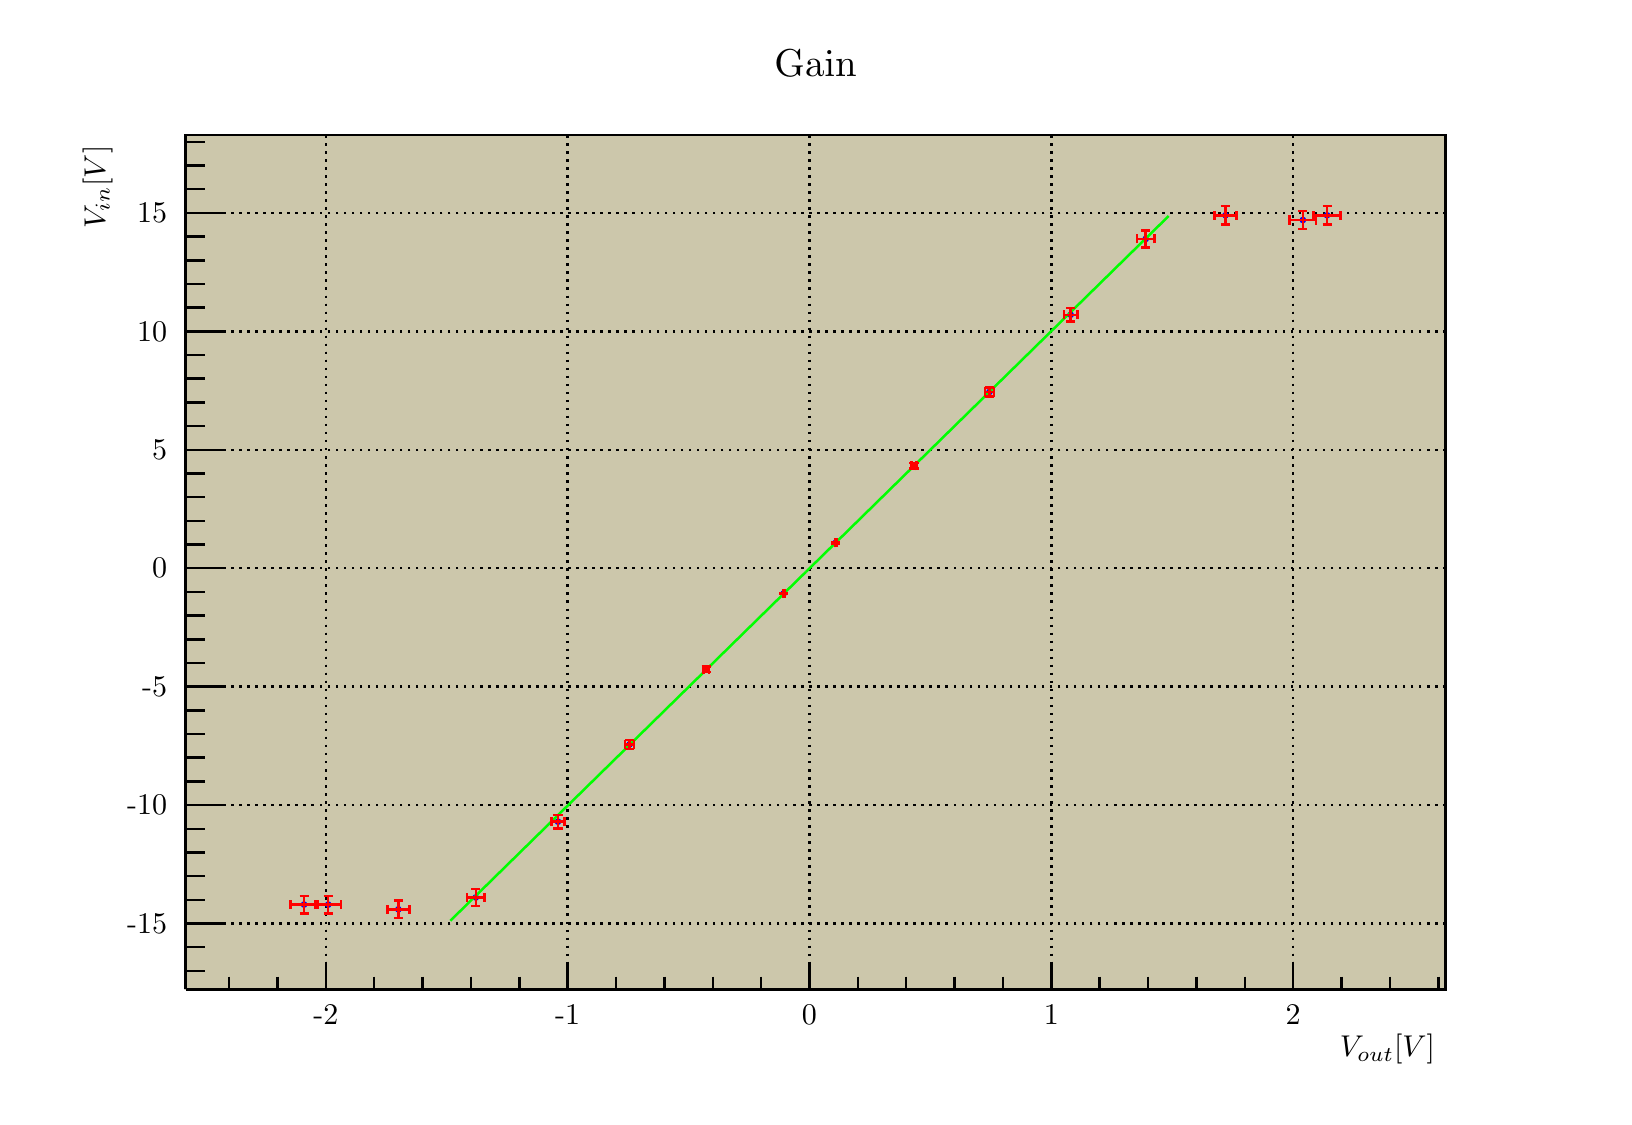
\begin{tikzpicture}
\pgfdeclareplotmark{cross} {
\pgfpathmoveto{\pgfpoint{-0.3\pgfplotmarksize}{\pgfplotmarksize}}
\pgfpathlineto{\pgfpoint{+0.3\pgfplotmarksize}{\pgfplotmarksize}}
\pgfpathlineto{\pgfpoint{+0.3\pgfplotmarksize}{0.3\pgfplotmarksize}}
\pgfpathlineto{\pgfpoint{+1\pgfplotmarksize}{0.3\pgfplotmarksize}}
\pgfpathlineto{\pgfpoint{+1\pgfplotmarksize}{-0.3\pgfplotmarksize}}
\pgfpathlineto{\pgfpoint{+0.3\pgfplotmarksize}{-0.3\pgfplotmarksize}}
\pgfpathlineto{\pgfpoint{+0.3\pgfplotmarksize}{-1.\pgfplotmarksize}}
\pgfpathlineto{\pgfpoint{-0.3\pgfplotmarksize}{-1.\pgfplotmarksize}}
\pgfpathlineto{\pgfpoint{-0.3\pgfplotmarksize}{-0.3\pgfplotmarksize}}
\pgfpathlineto{\pgfpoint{-1.\pgfplotmarksize}{-0.3\pgfplotmarksize}}
\pgfpathlineto{\pgfpoint{-1.\pgfplotmarksize}{0.3\pgfplotmarksize}}
\pgfpathlineto{\pgfpoint{-0.3\pgfplotmarksize}{0.3\pgfplotmarksize}}
\pgfpathclose
\pgfusepathqstroke
}
\pgfdeclareplotmark{cross*} {
\pgfpathmoveto{\pgfpoint{-0.3\pgfplotmarksize}{\pgfplotmarksize}}
\pgfpathlineto{\pgfpoint{+0.3\pgfplotmarksize}{\pgfplotmarksize}}
\pgfpathlineto{\pgfpoint{+0.3\pgfplotmarksize}{0.3\pgfplotmarksize}}
\pgfpathlineto{\pgfpoint{+1\pgfplotmarksize}{0.3\pgfplotmarksize}}
\pgfpathlineto{\pgfpoint{+1\pgfplotmarksize}{-0.3\pgfplotmarksize}}
\pgfpathlineto{\pgfpoint{+0.3\pgfplotmarksize}{-0.3\pgfplotmarksize}}
\pgfpathlineto{\pgfpoint{+0.3\pgfplotmarksize}{-1.\pgfplotmarksize}}
\pgfpathlineto{\pgfpoint{-0.3\pgfplotmarksize}{-1.\pgfplotmarksize}}
\pgfpathlineto{\pgfpoint{-0.3\pgfplotmarksize}{-0.3\pgfplotmarksize}}
\pgfpathlineto{\pgfpoint{-1.\pgfplotmarksize}{-0.3\pgfplotmarksize}}
\pgfpathlineto{\pgfpoint{-1.\pgfplotmarksize}{0.3\pgfplotmarksize}}
\pgfpathlineto{\pgfpoint{-0.3\pgfplotmarksize}{0.3\pgfplotmarksize}}
\pgfpathclose
\pgfusepathqfillstroke
}
\pgfdeclareplotmark{newstar} {
\pgfpathmoveto{\pgfqpoint{0pt}{\pgfplotmarksize}}
\pgfpathlineto{\pgfqpointpolar{44}{0.5\pgfplotmarksize}}
\pgfpathlineto{\pgfqpointpolar{18}{\pgfplotmarksize}}
\pgfpathlineto{\pgfqpointpolar{-20}{0.5\pgfplotmarksize}}
\pgfpathlineto{\pgfqpointpolar{-54}{\pgfplotmarksize}}
\pgfpathlineto{\pgfqpointpolar{-90}{0.5\pgfplotmarksize}}
\pgfpathlineto{\pgfqpointpolar{234}{\pgfplotmarksize}}
\pgfpathlineto{\pgfqpointpolar{198}{0.5\pgfplotmarksize}}
\pgfpathlineto{\pgfqpointpolar{162}{\pgfplotmarksize}}
\pgfpathlineto{\pgfqpointpolar{134}{0.5\pgfplotmarksize}}
\pgfpathclose
\pgfusepathqstroke
}
\pgfdeclareplotmark{newstar*} {
\pgfpathmoveto{\pgfqpoint{0pt}{\pgfplotmarksize}}
\pgfpathlineto{\pgfqpointpolar{44}{0.5\pgfplotmarksize}}
\pgfpathlineto{\pgfqpointpolar{18}{\pgfplotmarksize}}
\pgfpathlineto{\pgfqpointpolar{-20}{0.5\pgfplotmarksize}}
\pgfpathlineto{\pgfqpointpolar{-54}{\pgfplotmarksize}}
\pgfpathlineto{\pgfqpointpolar{-90}{0.5\pgfplotmarksize}}
\pgfpathlineto{\pgfqpointpolar{234}{\pgfplotmarksize}}
\pgfpathlineto{\pgfqpointpolar{198}{0.5\pgfplotmarksize}}
\pgfpathlineto{\pgfqpointpolar{162}{\pgfplotmarksize}}
\pgfpathlineto{\pgfqpointpolar{134}{0.5\pgfplotmarksize}}
\pgfpathclose
\pgfusepathqfillstroke
}
\definecolor{c}{rgb}{1,1,1};
\draw [color=c, fill=c] (0,0) rectangle (20,13.5632);
\definecolor{c}{rgb}{0.8,0.78,0.67};
\draw [color=c, fill=c] (2,1.35632) rectangle (18,12.2069);
\definecolor{c}{rgb}{0,0,0};
\draw [c,line width=0.9] (2,1.35632) -- (2,12.2069) -- (18,12.2069) -- (18,1.35632) -- (2,1.35632);
\definecolor{c}{rgb}{0.8,0.78,0.67};
\draw [color=c, fill=c] (2,1.35632) rectangle (18,12.2069);
\definecolor{c}{rgb}{0,0,0};
\draw [c,line width=0.9] (2,1.35632) -- (2,12.2069) -- (18,12.2069) -- (18,1.35632) -- (2,1.35632);
\draw [c,line width=0.9] (2,1.35632) -- (18,1.35632);
\draw [c,dotted,line width=0.9] (3.7792,12.2069) -- (3.7792,1.35632);
\draw [c,dotted,line width=0.9] (6.85062,12.2069) -- (6.85062,1.35632);
\draw [c,dotted,line width=0.9] (9.92204,12.2069) -- (9.92204,1.35632);
\draw [c,dotted,line width=0.9] (12.9935,12.2069) -- (12.9935,1.35632);
\draw [c,dotted,line width=0.9] (16.0649,12.2069) -- (16.0649,1.35632);
\draw [c,dotted,line width=0.9] (3.7792,12.2069) -- (3.7792,1.35632);
\draw [c,dotted,line width=0.9] (16.0649,12.2069) -- (16.0649,1.35632);
\draw [c,line width=0.9] (2,1.35632) -- (2,12.2069);
\draw [c,dotted,line width=0.9] (18,2.19282) -- (2,2.19282);
\draw [c,dotted,line width=0.9] (18,3.69696) -- (2,3.69696);
\draw [c,dotted,line width=0.9] (18,5.2011) -- (2,5.2011);
\draw [c,dotted,line width=0.9] (18,6.70524) -- (2,6.70524);
\draw [c,dotted,line width=0.9] (18,8.20938) -- (2,8.20938);
\draw [c,dotted,line width=0.9] (18,9.71352) -- (2,9.71352);
\draw [c,dotted,line width=0.9] (18,11.2177) -- (2,11.2177);
\draw [c,dotted,line width=0.9] (18,2.19282) -- (2,2.19282);
\draw [c,dotted,line width=0.9] (18,11.2177) -- (2,11.2177);
\draw [c,line width=0.9] (2,1.35632) -- (18,1.35632);
\draw [anchor= east] (18,0.596782) node[scale=1.08496, color=c, rotate=0]{$V_{out} [V]$};
\draw [c,line width=0.9] (3.7792,1.68184) -- (3.7792,1.35632);
\draw [c,line width=0.9] (4.39348,1.51908) -- (4.39348,1.35632);
\draw [c,line width=0.9] (5.00777,1.51908) -- (5.00777,1.35632);
\draw [c,line width=0.9] (5.62205,1.51908) -- (5.62205,1.35632);
\draw [c,line width=0.9] (6.23634,1.51908) -- (6.23634,1.35632);
\draw [c,line width=0.9] (6.85062,1.68184) -- (6.85062,1.35632);
\draw [c,line width=0.9] (7.46491,1.51908) -- (7.46491,1.35632);
\draw [c,line width=0.9] (8.07919,1.51908) -- (8.07919,1.35632);
\draw [c,line width=0.9] (8.69348,1.51908) -- (8.69348,1.35632);
\draw [c,line width=0.9] (9.30776,1.51908) -- (9.30776,1.35632);
\draw [c,line width=0.9] (9.92204,1.68184) -- (9.92204,1.35632);
\draw [c,line width=0.9] (10.5363,1.51908) -- (10.5363,1.35632);
\draw [c,line width=0.9] (11.1506,1.51908) -- (11.1506,1.35632);
\draw [c,line width=0.9] (11.7649,1.51908) -- (11.7649,1.35632);
\draw [c,line width=0.9] (12.3792,1.51908) -- (12.3792,1.35632);
\draw [c,line width=0.9] (12.9935,1.68184) -- (12.9935,1.35632);
\draw [c,line width=0.9] (13.6078,1.51908) -- (13.6078,1.35632);
\draw [c,line width=0.9] (14.222,1.51908) -- (14.222,1.35632);
\draw [c,line width=0.9] (14.8363,1.51908) -- (14.8363,1.35632);
\draw [c,line width=0.9] (15.4506,1.51908) -- (15.4506,1.35632);
\draw [c,line width=0.9] (16.0649,1.68184) -- (16.0649,1.35632);
\draw [c,line width=0.9] (3.7792,1.68184) -- (3.7792,1.35632);
\draw [c,line width=0.9] (3.16491,1.51908) -- (3.16491,1.35632);
\draw [c,line width=0.9] (2.55063,1.51908) -- (2.55063,1.35632);
\draw [c,line width=0.9] (16.0649,1.68184) -- (16.0649,1.35632);
\draw [c,line width=0.9] (16.6792,1.51908) -- (16.6792,1.35632);
\draw [c,line width=0.9] (17.2935,1.51908) -- (17.2935,1.35632);
\draw [c,line width=0.9] (17.9077,1.51908) -- (17.9077,1.35632);
\draw [anchor=base] (3.7792,0.908736) node[scale=1.08496, color=c, rotate=0]{-2};
\draw [anchor=base] (6.85062,0.908736) node[scale=1.08496, color=c, rotate=0]{-1};
\draw [anchor=base] (9.92204,0.908736) node[scale=1.08496, color=c, rotate=0]{0};
\draw [anchor=base] (12.9935,0.908736) node[scale=1.08496, color=c, rotate=0]{1};
\draw [anchor=base] (16.0649,0.908736) node[scale=1.08496, color=c, rotate=0]{2};
\draw [c,line width=0.9] (2,1.35632) -- (2,12.2069);
\draw [anchor= east] (0.88,12.2069) node[scale=1.08496, color=c, rotate=90]{$V_{in} [V]$};
\draw [c,line width=0.9] (2.48,2.19282) -- (2,2.19282);
\draw [c,line width=0.9] (2.24,2.49365) -- (2,2.49365);
\draw [c,line width=0.9] (2.24,2.79447) -- (2,2.79447);
\draw [c,line width=0.9] (2.24,3.0953) -- (2,3.0953);
\draw [c,line width=0.9] (2.24,3.39613) -- (2,3.39613);
\draw [c,line width=0.9] (2.48,3.69696) -- (2,3.69696);
\draw [c,line width=0.9] (2.24,3.99779) -- (2,3.99779);
\draw [c,line width=0.9] (2.24,4.29861) -- (2,4.29861);
\draw [c,line width=0.9] (2.24,4.59944) -- (2,4.59944);
\draw [c,line width=0.9] (2.24,4.90027) -- (2,4.90027);
\draw [c,line width=0.9] (2.48,5.2011) -- (2,5.2011);
\draw [c,line width=0.9] (2.24,5.50193) -- (2,5.50193);
\draw [c,line width=0.9] (2.24,5.80275) -- (2,5.80275);
\draw [c,line width=0.9] (2.24,6.10358) -- (2,6.10358);
\draw [c,line width=0.9] (2.24,6.40441) -- (2,6.40441);
\draw [c,line width=0.9] (2.48,6.70524) -- (2,6.70524);
\draw [c,line width=0.9] (2.24,7.00607) -- (2,7.00607);
\draw [c,line width=0.9] (2.24,7.30689) -- (2,7.30689);
\draw [c,line width=0.9] (2.24,7.60772) -- (2,7.60772);
\draw [c,line width=0.9] (2.24,7.90855) -- (2,7.90855);
\draw [c,line width=0.9] (2.48,8.20938) -- (2,8.20938);
\draw [c,line width=0.9] (2.24,8.51021) -- (2,8.51021);
\draw [c,line width=0.9] (2.24,8.81104) -- (2,8.81104);
\draw [c,line width=0.9] (2.24,9.11186) -- (2,9.11186);
\draw [c,line width=0.9] (2.24,9.41269) -- (2,9.41269);
\draw [c,line width=0.9] (2.48,9.71352) -- (2,9.71352);
\draw [c,line width=0.9] (2.24,10.0143) -- (2,10.0143);
\draw [c,line width=0.9] (2.24,10.3152) -- (2,10.3152);
\draw [c,line width=0.9] (2.24,10.616) -- (2,10.616);
\draw [c,line width=0.9] (2.24,10.9168) -- (2,10.9168);
\draw [c,line width=0.9] (2.48,11.2177) -- (2,11.2177);
\draw [c,line width=0.9] (2.48,2.19282) -- (2,2.19282);
\draw [c,line width=0.9] (2.24,1.89199) -- (2,1.89199);
\draw [c,line width=0.9] (2.24,1.59116) -- (2,1.59116);
\draw [c,line width=0.9] (2.48,11.2177) -- (2,11.2177);
\draw [c,line width=0.9] (2.24,11.5185) -- (2,11.5185);
\draw [c,line width=0.9] (2.24,11.8193) -- (2,11.8193);
\draw [c,line width=0.9] (2.24,12.1201) -- (2,12.1201);
\draw [anchor= east] (1.9,2.19282) node[scale=1.08496, color=c, rotate=0]{-15};
\draw [anchor= east] (1.9,3.69696) node[scale=1.08496, color=c, rotate=0]{-10};
\draw [anchor= east] (1.9,5.2011) node[scale=1.08496, color=c, rotate=0]{-5};
\draw [anchor= east] (1.9,6.70524) node[scale=1.08496, color=c, rotate=0]{0};
\draw [anchor= east] (1.9,8.20938) node[scale=1.08496, color=c, rotate=0]{5};
\draw [anchor= east] (1.9,9.71352) node[scale=1.08496, color=c, rotate=0]{10};
\draw [anchor= east] (1.9,11.2177) node[scale=1.08496, color=c, rotate=0]{15};
\definecolor{c}{rgb}{0,0,1};
\foreach \P in {(13.2392,9.9241), (6.72776,3.48638), (10.2538,7.02712), (9.5934,6.38335), (11.2489,8.00482), (8.61055,5.4207), (12.2072,8.9434), (7.63691,4.46708), (14.1913,10.8867), (5.68348,2.52373), (15.2049,11.1876), (4.70063,2.37331),
 (16.1877,11.1274), (3.80991,2.43348), (16.4949,11.1876), (3.50277,2.43348)}{\draw[mark options={color=c,fill=c},mark size=1.681682pt,mark=*,mark size=1pt] plot coordinates {\P};}
\definecolor{c}{rgb}{0,1,0};
\draw [c,line width=0.9] (5.36098,2.22861) -- (5.45312,2.319) -- (5.54527,2.4094) -- (5.63741,2.4998) -- (5.72955,2.59019) -- (5.82169,2.68059) -- (5.91384,2.77099) -- (6.00598,2.86138) -- (6.09812,2.95178) -- (6.19027,3.04218) -- (6.28241,3.13257)
 -- (6.37455,3.22297) -- (6.46669,3.31337) -- (6.55884,3.40376) -- (6.65098,3.49416) -- (6.74312,3.58456) -- (6.83526,3.67495) -- (6.92741,3.76535) -- (7.01955,3.85575) -- (7.11169,3.94614) -- (7.20384,4.03654) -- (7.29598,4.12694) --
 (7.38812,4.21733) -- (7.48026,4.30773) -- (7.57241,4.39812) -- (7.66455,4.48852) -- (7.75669,4.57892) -- (7.84883,4.66931) -- (7.94098,4.75971) -- (8.03312,4.85011) -- (8.12526,4.9405) -- (8.21741,5.0309) -- (8.30955,5.1213) -- (8.40169,5.21169) --
 (8.49383,5.30209) -- (8.58598,5.39249) -- (8.67812,5.48288) -- (8.77026,5.57328) -- (8.8624,5.66368) -- (8.95455,5.75407) -- (9.04669,5.84447) -- (9.13883,5.93487) -- (9.23098,6.02526) -- (9.32312,6.11566) -- (9.41526,6.20606) -- (9.5074,6.29645) --
 (9.59955,6.38685) -- (9.69169,6.47725) -- (9.78383,6.56764) -- (9.87597,6.65804);
\draw [c,line width=0.9] (9.87597,6.65804) -- (9.96812,6.74844) -- (10.0603,6.83883) -- (10.1524,6.92923) -- (10.2445,7.01963) -- (10.3367,7.11002) -- (10.4288,7.20042) -- (10.521,7.29082) -- (10.6131,7.38121) -- (10.7053,7.47161) --
 (10.7974,7.56201) -- (10.8895,7.6524) -- (10.9817,7.7428) -- (11.0738,7.8332) -- (11.166,7.92359) -- (11.2581,8.01399) -- (11.3503,8.10439) -- (11.4424,8.19478) -- (11.5345,8.28518) -- (11.6267,8.37558) -- (11.7188,8.46597) -- (11.811,8.55637) --
 (11.9031,8.64677) -- (11.9953,8.73716) -- (12.0874,8.82756) -- (12.1795,8.91796) -- (12.2717,9.00835) -- (12.3638,9.09875) -- (12.456,9.18915) -- (12.5481,9.27954) -- (12.6403,9.36994) -- (12.7324,9.46034) -- (12.8245,9.55073) -- (12.9167,9.64113)
 -- (13.0088,9.73153) -- (13.101,9.82192) -- (13.1931,9.91232) -- (13.2853,10.0027) -- (13.3774,10.0931) -- (13.4695,10.1835) -- (13.5617,10.2739) -- (13.6538,10.3643) -- (13.746,10.4547) -- (13.8381,10.5451) -- (13.9303,10.6355) -- (14.0224,10.7259)
 -- (14.1145,10.8163) -- (14.2067,10.9067) -- (14.2988,10.9971) -- (14.391,11.0875);
\draw [c,line width=0.9] (14.391,11.0875) -- (14.4831,11.1779);
\definecolor{c}{rgb}{1,0,0};
\draw [c,line width=0.9] (13.2392,9.9241) -- (13.1528,9.9241);
\draw [c,line width=0.9] (13.1528,9.86663) -- (13.1528,9.98157);
\draw [c,line width=0.9] (13.2392,9.9241) -- (13.3255,9.9241);
\draw [c,line width=0.9] (13.3255,9.86663) -- (13.3255,9.98157);
\draw [c,line width=0.9] (13.2392,9.9241) -- (13.2392,10.0082);
\draw [c,line width=0.9] (13.1817,10.0082) -- (13.2967,10.0082);
\draw [c,line width=0.9] (13.2392,9.9241) -- (13.2392,9.83998);
\draw [c,line width=0.9] (13.1817,9.83998) -- (13.2967,9.83998);
\draw [c,line width=0.9] (6.72776,3.48638) -- (6.64328,3.48638);
\draw [c,line width=0.9] (6.64328,3.42891) -- (6.64328,3.54385);
\draw [c,line width=0.9] (6.72776,3.48638) -- (6.81225,3.48638);
\draw [c,line width=0.9] (6.81225,3.42891) -- (6.81225,3.54385);
\draw [c,line width=0.9] (6.72776,3.48638) -- (6.72776,3.5705);
\draw [c,line width=0.9] (6.67029,3.5705) -- (6.78524,3.5705);
\draw [c,line width=0.9] (6.72776,3.48638) -- (6.72776,3.40226);
\draw [c,line width=0.9] (6.67029,3.40226) -- (6.78524,3.40226);
\draw [c,line width=0.9] (10.2538,7.02712) -- (10.2451,7.02712);
\draw [c,line width=0.9] (10.2451,6.96965) -- (10.2451,7.0846);
\draw [c,line width=0.9] (10.2538,7.02712) -- (10.2624,7.02712);
\draw [c,line width=0.9] (10.2624,6.96965) -- (10.2624,7.0846);
\draw [c,line width=0.9] (10.2538,7.02712) -- (10.2538,7.03554);
\draw [c,line width=0.9] (10.1963,7.03554) -- (10.3112,7.03554);
\draw [c,line width=0.9] (10.2538,7.02712) -- (10.2538,7.01871);
\draw [c,line width=0.9] (10.1963,7.01871) -- (10.3112,7.01871);
\draw [c,line width=0.9] (9.5934,6.38335) -- (9.58481,6.38335);
\draw [c,line width=0.9] (9.58481,6.32588) -- (9.58481,6.44082);
\draw [c,line width=0.9] (9.5934,6.38335) -- (9.60199,6.38335);
\draw [c,line width=0.9] (9.60199,6.32588) -- (9.60199,6.44082);
\draw [c,line width=0.9] (9.5934,6.38335) -- (9.5934,6.39176);
\draw [c,line width=0.9] (9.53593,6.39176) -- (9.65087,6.39176);
\draw [c,line width=0.9] (9.5934,6.38335) -- (9.5934,6.37494);
\draw [c,line width=0.9] (9.53593,6.37494) -- (9.65087,6.37494);
\draw [c,line width=0.9] (11.2489,8.00482) -- (11.2144,8.00482);
\draw [c,line width=0.9] (11.2144,7.94734) -- (11.2144,8.06229);
\draw [c,line width=0.9] (11.2489,8.00482) -- (11.2834,8.00482);
\draw [c,line width=0.9] (11.2834,7.94734) -- (11.2834,8.06229);
\draw [c,line width=0.9] (11.2489,8.00482) -- (11.2489,8.03865);
\draw [c,line width=0.9] (11.1914,8.03865) -- (11.3064,8.03865);
\draw [c,line width=0.9] (11.2489,8.00482) -- (11.2489,7.97098);
\draw [c,line width=0.9] (11.1914,7.97098) -- (11.3064,7.97098);
\draw [c,line width=0.9] (8.61055,5.4207) -- (8.57624,5.4207);
\draw [c,line width=0.9] (8.57624,5.36323) -- (8.57624,5.47817);
\draw [c,line width=0.9] (8.61055,5.4207) -- (8.64486,5.4207);
\draw [c,line width=0.9] (8.64486,5.36323) -- (8.64486,5.47817);
\draw [c,line width=0.9] (8.61055,5.4207) -- (8.61055,5.45431);
\draw [c,line width=0.9] (8.55308,5.45431) -- (8.66802,5.45431);
\draw [c,line width=0.9] (8.61055,5.4207) -- (8.61055,5.3871);
\draw [c,line width=0.9] (8.55308,5.3871) -- (8.66802,5.3871);
\draw [c,line width=0.9] (12.2072,8.9434) -- (12.1485,8.9434);
\draw [c,line width=0.9] (12.1485,8.88593) -- (12.1485,9.00087);
\draw [c,line width=0.9] (12.2072,8.9434) -- (12.2659,8.9434);
\draw [c,line width=0.9] (12.2659,8.88593) -- (12.2659,9.00087);
\draw [c,line width=0.9] (12.2072,8.9434) -- (12.2072,9.00091);
\draw [c,line width=0.9] (12.1497,9.00091) -- (12.2647,9.00091);
\draw [c,line width=0.9] (12.2072,8.9434) -- (12.2072,8.88589);
\draw [c,line width=0.9] (12.1497,8.88589) -- (12.2647,8.88589);
\draw [c,line width=0.9] (7.63691,4.46708) -- (7.57819,4.46708);
\draw [c,line width=0.9] (7.57819,4.40961) -- (7.57819,4.52455);
\draw [c,line width=0.9] (7.63691,4.46708) -- (7.69562,4.46708);
\draw [c,line width=0.9] (7.69562,4.40961) -- (7.69562,4.52455);
\draw [c,line width=0.9] (7.63691,4.46708) -- (7.63691,4.52458);
\draw [c,line width=0.9] (7.57943,4.52458) -- (7.69438,4.52458);
\draw [c,line width=0.9] (7.63691,4.46708) -- (7.63691,4.40957);
\draw [c,line width=0.9] (7.57943,4.40957) -- (7.69438,4.40957);
\draw [c,line width=0.9] (14.1913,10.8867) -- (14.0785,10.8867);
\draw [c,line width=0.9] (14.0785,10.8293) -- (14.0785,10.9442);
\draw [c,line width=0.9] (14.1913,10.8867) -- (14.3041,10.8867);
\draw [c,line width=0.9] (14.3041,10.8293) -- (14.3041,10.9442);
\draw [c,line width=0.9] (14.1913,10.8867) -- (14.1913,10.9972);
\draw [c,line width=0.9] (14.1339,10.9972) -- (14.2488,10.9972);
\draw [c,line width=0.9] (14.1913,10.8867) -- (14.1913,10.7763);
\draw [c,line width=0.9] (14.1339,10.7763) -- (14.2488,10.7763);
\draw [c,line width=0.9] (5.68348,2.52373) -- (5.57114,2.52373);
\draw [c,line width=0.9] (5.57114,2.46626) -- (5.57114,2.5812);
\draw [c,line width=0.9] (5.68348,2.52373) -- (5.79582,2.52373);
\draw [c,line width=0.9] (5.79582,2.46626) -- (5.79582,2.5812);
\draw [c,line width=0.9] (5.68348,2.52373) -- (5.68348,2.63421);
\draw [c,line width=0.9] (5.62601,2.63421) -- (5.74095,2.63421);
\draw [c,line width=0.9] (5.68348,2.52373) -- (5.68348,2.41324);
\draw [c,line width=0.9] (5.62601,2.41324) -- (5.74095,2.41324);
\draw [c,line width=0.9] (15.2049,11.1876) -- (15.0647,11.1876);
\draw [c,line width=0.9] (15.0647,11.1301) -- (15.0647,11.245);
\draw [c,line width=0.9] (15.2049,11.1876) -- (15.3451,11.1876);
\draw [c,line width=0.9] (15.3451,11.1301) -- (15.3451,11.245);
\draw [c,line width=0.9] (15.2049,11.1876) -- (15.2049,11.3027);
\draw [c,line width=0.9] (15.1474,11.3027) -- (15.2624,11.3027);
\draw [c,line width=0.9] (15.2049,11.1876) -- (15.2049,11.0725);
\draw [c,line width=0.9] (15.1474,11.0725) -- (15.2624,11.0725);
\draw [c,line width=0.9] (4.70063,2.37331) -- (4.56136,2.37331);
\draw [c,line width=0.9] (4.56136,2.31584) -- (4.56136,2.43079);
\draw [c,line width=0.9] (4.70063,2.37331) -- (4.83989,2.37331);
\draw [c,line width=0.9] (4.83989,2.31584) -- (4.83989,2.43079);
\draw [c,line width=0.9] (4.70063,2.37331) -- (4.70063,2.48609);
\draw [c,line width=0.9] (4.64315,2.48609) -- (4.7581,2.48609);
\draw [c,line width=0.9] (4.70063,2.37331) -- (4.70063,2.26054);
\draw [c,line width=0.9] (4.64315,2.26054) -- (4.7581,2.26054);
\draw [c,line width=0.9] (16.1877,11.1274) -- (16.0206,11.1274);
\draw [c,line width=0.9] (16.0206,11.0699) -- (16.0206,11.1849);
\draw [c,line width=0.9] (16.1877,11.1274) -- (16.3549,11.1274);
\draw [c,line width=0.9] (16.3549,11.0699) -- (16.3549,11.1849);
\draw [c,line width=0.9] (16.1877,11.1274) -- (16.1877,11.2416);
\draw [c,line width=0.9] (16.1303,11.2416) -- (16.2452,11.2416);
\draw [c,line width=0.9] (16.1877,11.1274) -- (16.1877,11.0132);
\draw [c,line width=0.9] (16.1303,11.0132) -- (16.2452,11.0132);
\draw [c,line width=0.9] (3.80991,2.43348) -- (3.64508,2.43348);
\draw [c,line width=0.9] (3.64508,2.37601) -- (3.64508,2.49095);
\draw [c,line width=0.9] (3.80991,2.43348) -- (3.97474,2.43348);
\draw [c,line width=0.9] (3.97474,2.37601) -- (3.97474,2.49095);
\draw [c,line width=0.9] (3.80991,2.43348) -- (3.80991,2.54534);
\draw [c,line width=0.9] (3.75244,2.54534) -- (3.86738,2.54534);
\draw [c,line width=0.9] (3.80991,2.43348) -- (3.80991,2.32162);
\draw [c,line width=0.9] (3.75244,2.32162) -- (3.86738,2.32162);
\draw [c,line width=0.9] (16.4949,11.1876) -- (16.3231,11.1876);
\draw [c,line width=0.9] (16.3231,11.1301) -- (16.3231,11.245);
\draw [c,line width=0.9] (16.4949,11.1876) -- (16.6667,11.1876);
\draw [c,line width=0.9] (16.6667,11.1301) -- (16.6667,11.245);
\draw [c,line width=0.9] (16.4949,11.1876) -- (16.4949,11.3027);
\draw [c,line width=0.9] (16.4374,11.3027) -- (16.5524,11.3027);
\draw [c,line width=0.9] (16.4949,11.1876) -- (16.4949,11.0725);
\draw [c,line width=0.9] (16.4374,11.0725) -- (16.5524,11.0725);
\draw [c,line width=0.9] (3.50277,2.43348) -- (3.33333,2.43348);
\draw [c,line width=0.9] (3.33333,2.37601) -- (3.33333,2.49095);
\draw [c,line width=0.9] (3.50277,2.43348) -- (3.67221,2.43348);
\draw [c,line width=0.9] (3.67221,2.37601) -- (3.67221,2.49095);
\draw [c,line width=0.9] (3.50277,2.43348) -- (3.50277,2.54534);
\draw [c,line width=0.9] (3.4453,2.54534) -- (3.56024,2.54534);
\draw [c,line width=0.9] (3.50277,2.43348) -- (3.50277,2.32162);
\draw [c,line width=0.9] (3.4453,2.32162) -- (3.56024,2.32162);
\definecolor{c}{rgb}{0,0,0};
\draw (10,13.1224) node[scale=1.40406, color=c, rotate=0]{Gain};
\end{tikzpicture}
 
 \caption{Curva di trasferimento di un amplificatore invertente} 
 \label{gr:amp_noninv.tex} 
\end{grafico}

\begin{tabella}
 \centering
 \begin{center}
\begin{tabulary}{\textwidth}{CCCCCC}
\toprule
$V_{in+}$ (V) & $V_{in-}$ (V) & FS (V) & $V_{out+}$(V) & $V_{out-}$ (V) & FS (V) \\ \midrule 
1.08 & -1.04 & 0.3 & 10.7 & -10.7 & 3 \\ \midrule
0.108 & -0.107 & 0.03 & 1.07 & -1.07 & 0.3 \\ \midrule
0.432 & -0.427 & 0.120 & 4.32 & -4.27 & 1.2 \\ \midrule
0.744 & -0.744 & 0.2 & 7.44 & -7.44 & 2 \\ \midrule 
1.39 & -1.38 & 0.4 & 13.9 & -13.9 & 4 \\ \midrule
1.72 & -1.70 & 0.5 & 14.9 & -14.4 & 4 \\ \midrule
2.04 & -1.99 & 0.6 & 14.7 & -14.2 & 4 \\ \midrule
2.14 & -2.09 & 0.6 & 14.9 & -14.2 & 4 \\ \midrule


\bottomrule
\end{tabulary}
\end{center}
 
 \caption{Dati curva di trasferimento}
 \label{tab:tab_non_inv.tex}
\end{tabella}

E' stata fatta l'interpolazione lineare pesata dei punti compresi tra 0 e 1.5 V.
%retta interpolazione

